\documentclass{resume} % Use the custom resume.cls style
\usepackage{graphicx}
\usepackage{hyperref}

\usepackage[left=0.75in,top=0.6in,right=0.75in,bottom=0.6in]{geometry} % Document margins
\newcommand{\tab}[1]{\hspace{.2667\textwidth}\rlap{#1}}
\newcommand{\itab}[1]{\hspace{0em}\rlap{#1}}

\name{Karthik P Bilichod} % Your name

\begin{document}


\begin{rSection}{ }

H.No-605, 17th main, 10th cross \hfill  Contact No. : 8971278593 \\
Padmanabhanagar  \hfill Email ID : karthikpk23@gmail.com \\
Bengaluru - 560070\\
Karnataka\\
\end{rSection}

\begin{center}
\hspace{10 cm}
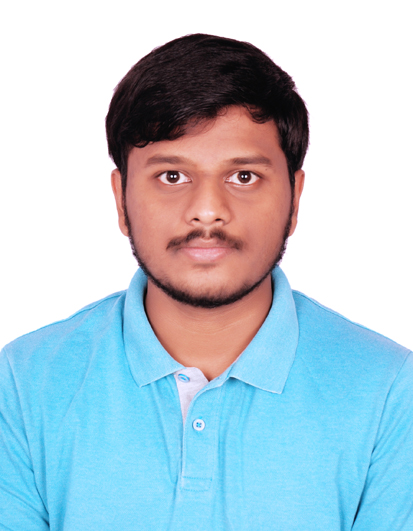
\includegraphics{karthik}
\end{center}

\vskip 0.5in

\begin{rSection}{Objective}
 I am interested to work in the field of Embedded systems, Robotics(especially aerial robotics), RF and Antennas. I will definitely work hard and give my best to solve problems which will help the society.
\end{rSection}

\vskip 0.5in

\begin{rSection}{Education}
\centering
\begin{tabular}{|l|l|l|l|l|}
\hline
{\bf Course} & {\bf Discipline} & {\bf Institution} & {\bf Year of passing} & {\bf Score} \\
&&&&\\
\hline
 School & Class-10th CBSE & Kendriya Vidyalaya Hospet & 2014 & 9.6 CGPA\\
 &&&&\\
 \hline
 Pre University & Class-12th CBSE & Sharada Vidyaniketana & 2016 & 92.25(PCMB)\\
  & & Public School & &Percent\\
  && Mangaluru &&\\
  \hline
  B.Tech & Electronics and & PES University & 2020 & 8.3 CGPA\\
  &Communication& Bengaluru &&Sem 1 to Sem 5\\
  & Engineering&&&\\
  \hline
\end{tabular}
\end{rSection}

\pagebreak

\begin{rSection}{Projects}
\begin{enumerate}
    \item {\bf Ball catching Robot} during Summer internship at {\bf Microsoft Innovation Lab} PES University under the guidance of Dr.Venkatarangan MJ and Prof Rajasekar M. Used Firebird-V platform for catching and OpenCV for trajectory prediction.
    \item {\bf Self balancing Robot} using PID control as a mini project for the course {\bf Introduction to Robotics} under the guidance of Dr.Venkatrangan MJ.
    \item Faster computation of {\bf Inverse of huge matrices} using recurrent neural networks as a mini project for course {\bf Machine Learning} under the guidance of Dr.Koshy K George.{\bf (In progress)}
    \item {\bf Determination of array factor for Superdirective characterstics} as a research project under the guidance of Dr.Saumya Adhikari.
    \item A {\bf Drone} for Defence applications as a hobby project.{\bf (In progress)}
    \item Establishing fast communication between multiple ESP32 modules using {\bf WiFi Direct} (without internet)  under the guidance of Dr.Manikandan J at {\bf Crucible of Research and Innovation}, PES University.
    \item {\bf Sun tracking solar panel} using AT89C51 microcontroller and LDRs as a mini project for the course {\bf Microcontrollers}.
    \item {\bf Cell Phone Detector} using LM358 Dual OpAmp as a mini project for the course {\bf Linear Integrated Circuits}.
    \item {\bf Fruit Plucking Robot} for JED-I(Joy of Engineering Design and Innovation) lab using Arduino Uno and image processing using OpenCV.
\end{enumerate}
\end{rSection}

\vskip 0.5in

\begin{rSection}{Training and Internships}
\begin{itemize}
    \item {\bf PNM Satellite Design course} held at PES University by Prof. Sharan Asundi from Tuskegee University.
    \item {\bf Compu music} course to produce and compose music using software Chuck.
    \item {\bf IoT workshop} held at PES University by i3indya technologies.
    \item Interned at {\bf CORI}( Crucible of Research and Innovation), PES University.
    \item Interned at {\bf Microsoft Innovation Lab}, PES University.\\

\end{itemize}
\end{rSection}

\vskip 0.5in

\begin{rSection}{Research Publications}
\begin{enumerate}
    \item {\bf To synthesize an Array Factor for Superdirective chracterstics of a broadside Antenna}. Have successfully completed and finalized the array factor and the work is about to be published. It is being done under the guidance of {\bf Dr.Saumya Adhikari}.\\
\end{enumerate}
\end{rSection}

\pagebreak

\begin{rSection}{Technical skills}
\begin{itemize}
    \item {\bf Programming languages :} \\
     C, C++, Python, Matlab.
     \item {\bf Software worked with :} \\
     Atmel studio 6, Arduino IDE, Scilab, MATLAB, keiluvision 3, XCTU, Blender Animation.
     \item {\bf Hardware worked with :} \\
     Arduino Uno and NANO, Firebird V robot with ATmega 2560 microcontroller, Xbee Modules, ESP32 Wifi Module, Various sensor interfaces.
     
     \item {\bf OS worked in :} \\
     Ubuntu , Microsoft Windows 7/8/10 ,XP
\end{itemize}
\end{rSection}

\vskip 0.5in

\begin{rSection}{Soft skills}
\begin{enumerate}
    \item Hard working and Resilient.
    \item Helping Nature.
    \item Good leadership qualities.
    \item Good in team work.
    \item Languages spoken: Kannada, English, Hindi, Telugu.
\end{enumerate}
\end{rSection}

\vskip 0.5in

\begin{rSection}{Extra - Curricular Activities}
\begin{itemize}
    \item Attended Foreign language courses. Opted and passed in German language course from PES University.
    \item Tabla and keyboard player.
    \item Basketball and Badminton player.
    \item Learning Sanskrit and reading ancient Indian texts in Sanskrit.
\end{itemize}
\end{rSection}

\vskip 0.5in


\begin{rSection}{Co - Curricular Activities}
\begin{enumerate}
    \item Attend many talks and guest lectures. Attended the talk of 2017 Nobel Laureate {\bf Kip Thorne} at ICTS, Bangalore on 11th Jan 2018.
    \item Participated and won third prize in college technical fest {\bf Prakalpa}.
    \item Participated in Eyantra Robotics Competition 2017 and 2018. Certificate of completion in 2017 and finalists in 2018. 
    \item Have done Mini projects based on regular courses to understand practical aspects of course work.
\end{enumerate}
\end{rSection}

\pagebreak

\begin{rSection}{Personal details}
Father's Name : B S Prasanna \\
Mother's Name : B Srusti \\
Sex : Male \\
Date of Birth : 28th January 1999 \\
Nationality : Indian \\
\end{rSection}

\begin{rSection}{Reference}
\begin{itemize}
	\item Dr.Saumya Adhikari\\
		Professor, Electronics and Communication Department\\
		PES University, Bengaluru\\
		Email ID : \href {https://faculty.pes.edu/p10110}{saumya.adhikari@pes.edu} \\

	\item Dr.Venkatarangan MJ\\
		Professor, Electrical and Electronics Department\\
		PES University, Bengaluru\\
		Email ID : \href{http://13.232.26.175/p10106}{venkataranganmj@pes.edu} \\

	\item Prof Rajasekar M\\
		Associate Professor, Electronics and Communication Department\\
		PES University, Bengaluru\\
		Email ID :  \href{https://faculty.pes.edu/p10125}{rajasekarmohan@pes.edu} \\
\end{itemize}
\end{rSection}

\begin{rSection}{Declaration}
I hereby declare that above-mentioned information is correct to the best of my knowledge and belief. \\
\end{rSection}

{\bf Date : } 15th April 2019

\end{document}

